\documentclass[12pt]{amsart}
\usepackage{amsthm}
\usepackage{graphicx}
\newcommand*\oct{\vcenter{\hbox{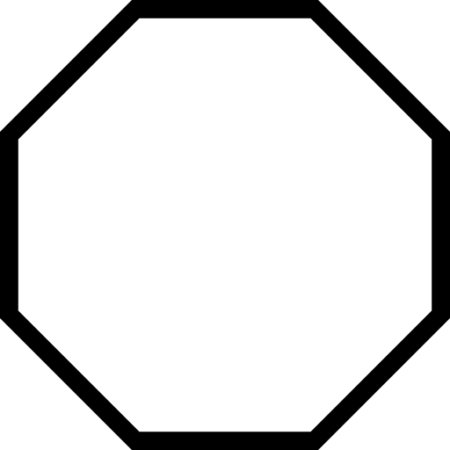
\includegraphics[width=.9em]{octagon.png}}}}
\newcommand{\F}{\mathcal{F}}
\newcommand{\Z}{\mathbb{Z}}

\newtheorem{theorem}{Theorem}
\newtheorem{lemma}{Lemma}
\newtheorem{proposition}{Proposition}
\newtheorem{corollary}{Corollary}

\theoremstyle{definition}
\newtheorem{definition}{Definition}

\title{Stopping Times}
\author{Robert Dougherty-Bliss and Charles Kenney}

\begin{document}
\maketitle

\section{Stopped binary strings}
\label{sec:stopped_binary_strings}

\begin{definition}
    A \emph{binary string of length $n$} is a tuple $(x_1, x_2, \dots, x_n)$
    where each $x_k$ is $0$ or $1$. Such a string is said to be \emph{stopped}
    at index $k$ if every index of the tuple in $(k / 2, k]$ is zero. The
    \emph{stopping time} of a binary string is the smallest $k$ such that the
    string is stopped at index $k$, or $\infty$ if no such $k$ exists. Note
    that, except $1$ and $\infty$, every stopping time is even.
\end{definition}

We should first note that this definition and our later results generalize
immediately to bases other than $2$. The only change in the definition is that
the elements of the strings may be anything in $\{0, 1, \dots, b - 1\}$ in base
$b$. In the later arguments, ``$1$'' should be replaced with ``any nonzero
number.''  For simplicity we will sometimes discuss only binary, but will quote
the arbitrary base results when they are needed.

We are primarily interested in binary strings of length $n$ which have stopping
time $n$. Indeed, let $g(n)$ be the number of such strings. Our first goal is
to show that $g(n)$ satifies the recurrence
\begin{align*}
    g(1) &= g(2) = g(4) = 1 \\
    g(4n) &= 2 g(4n - 2) \\
    g(4n + 2) &= 2 g(4n) - g(2n).
\end{align*}
This will identify the sequence $a(n) = g(2n)$ as the
\emph{Narayana--Zidek--Capell numbers}, A2083 in the OEIS, which begin
\begin{equation*}
    1, 1, 1, 2, 3, 6, 11, 22, 42, 84, 165, 330, 654, \dots
\end{equation*}
This recurrence was discovered thanks to the OEIS.

Our first definition discusses \emph{finite} binary strings, but it is more
convenient to work with \emph{infinite} binary strings which are nonzero in
only finitely many places. This is equivalent, and has the benefit that every
such infinite string has a finite stopping time when considered as a
sufficiently long, finite binary string.

\begin{definition}
    Let
    \begin{equation*}
        V = \bigoplus_{k=1}^\infty (\Z/2\Z)
    \end{equation*}
    be the direct sum of infinitely many copies of $\Z / 2\Z$. That is, the set
    of all infinite tuples $(x_1, x_2, x_3, \dots)$ where each $x_k$ is $0$ or
    $1$, and only finitely many are $1$. For each positive integer $k$, let
    $\oct_k$ be the set of elements of $V$ which are zero beyond position $k$
    and, when the first $k$ entries are regarded as a finite binary string,
    they have stopping time $k$. That is, $\oct_1 = \{0\} \subset V$,
    \begin{equation*}
        \oct_{2k} = \{v \in V : \forall j > k, v_j = 0, \text{ and } v \text{ has stopping time } 2k \}
    \end{equation*}
    and $\oct_{2k + 1} = \emptyset$ for every integer $k \geq 1$.
\end{definition}

It is clear that $g(n) = |\oct_n|$ for every positive integer $n$.

\begin{theorem}
    The sequence $g(n)$ satisfies the recurrence
    \begin{align*}
        g(1) &= g(2) = g(4) = 1 \\
        g(4n) &= 2 g(4n - 2) \\
        g(4n + 2) &= 2 g(4n) - g(2n).
    \end{align*}
\end{theorem}

\begin{proof} \textit{(1)}
    Each nonzero element in $V$ has a final nonzero entry (a one). Let $e_0 \colon V
    \to V$ be a map which inserts a $0$ in the position of this final entry,
    shifting the previous final entry to the right one space. Similarly, let $e_1$ insert a $1$.
    Symbolically,
    \begin{equation*}
        e_0(b) =
            \begin{cases}
                0 \text{ if } b=0 \\
                (b_1, ..., b_j, 0, 1, 0,0,...) \text{ if } b = (b_1, ..., b_j, 1, 0, 0, ...)
            \end{cases}
    \end{equation*}
    and
    \begin{equation*}
        e_1(b) =
            \begin{cases}
                (1, 0, 0, \dots) \text{ if } b=0 \\
                (b_1, ..., b_j, 1, 1, 0,0,...) \text{ if } b = (b_1, ..., b_j, 1, 0, 0, ...).
            \end{cases}
    \end{equation*}
    Note that $e_0$ and $e_1$ are injective, $e_0(V) \cap e_1(V) = \emptyset,$
    and $e_0(V) \cup e_1(V) = V.$

    For any positive integer $k$,
    \begin{equation*}
        \oct_{2k + 2} \subseteq e_0(\oct_{2k}) \cup e_1(\oct_{2k}).
    \end{equation*}
    Indeed, the final nonzero entry of every string in $\oct_{2k + 2}$ occurs
    at position $k + 1$. Removing the immediately preceding entry produces a
    string in $\oct_{2k}$---$e_0$ and $e_1$ simply add the entry back.

    In the other direction, for $k \geq 2$ we have
    \begin{equation*}
        e_1(\oct_{2k}) \subseteq \oct_{2k + 2},
    \end{equation*}
    because inserting a $1$ into position $k$ will never decrease the stopping
    time. For \emph{odd} $k \geq 3$ we have
    \begin{equation*}
        e_0(\oct_{2k}) \subseteq \oct_{2k + 2},
    \end{equation*}
    because inserting a $0$ at position $k$ will only decrease the stopping
    time if the new stopping time \emph{is} $k$; this is impossible if $k$ is
    odd. This shows that
    \begin{equation*}
        \oct_{2k + 2} = e_0(\oct_{2k}) \cup e_1(\oct_{2k}),
    \end{equation*}
    and thus
    \begin{equation*}
        g(2k + 2) = 2 g(2k)
    \end{equation*}
    for $k$ odd.

    To handle the even case, let
    \begin{equation*}
        \oct_{2k}^1 = \{(b_1, ..., b_{2k}, 1, 0,0,...) \in V \text{ s.t. } (b_1,...,b_{2k},0,0,...) \in \oct_{2k}\}.
    \end{equation*}
    (Note that $|\oct_{2k}^1| = |\oct_{2k}| = g(2k)$.) Then
    \begin{equation*}
        e_0(\oct_{4k}) \subseteq \oct_{4k + 2} \cup \oct_{2k}^1.
    \end{equation*}
    This implies
    \begin{equation*}
        \oct_{4k + 2} \cup \oct_{2k}^1 = e_0(\oct_{4k}) \cup e_1(\oct_{4k}).
    \end{equation*}
    (That the left contains the right is clear given the preceding inclusion.
    For the other direction, note $\oct_{2k}^1 \subseteq
    e_0(\oct_{4k})$, since if $(b_1, ..., b_{2k}, 0,0,...) \in \oct_{2k}$ then
    $(b_1, ..., b_{2k-1},1,0,0,...)$ has stopping time precisely $4k$.) Therefore
    \begin{equation*}
        g(4k + 2) + |\oct_{2k}^1| = 2 g(4k),
    \end{equation*}
    or
    \begin{equation*}
        g(4k + 2) = 2 g(4k) - g(2k).
    \end{equation*}
    This establishes the recurrence.
\end{proof}

\begin{proof} \textit{(2)}
    \begin{definition}
        A \emph{composition} of $n$ is a vector in $(\Z_{>0})^m$, for some $m \in \{1,2,...,n\},$ whose components add to $n$.
    \end{definition}
    The $n$th Narayana-Zidek-Capell number, $a(n),$ is the cardinality of the set
    \begin{align*}
        R_n = \left\{ \text{Compositions } p \text{ of } n \text{ satisfying } p_1 = 1 \text{ and } p_k \leq \sum_{j=1}^{k-1} p_j \right\}.
    \end{align*}
    %OEIS reference for this, or better yet the original source
    For $j \in \Z_{>0},$ let $f(j) = (0,0,...,0,1)$, with $j-1$ zeroes preceding the one.
    Then for $p \in (\Z_{>0})^m,$ let
    \begin{align*}
        F(p) = (f(p_1), f(p_2), ..., f(p_m), 0,0,...),
    \end{align*}
    concatenated in the natural way, with a tail of zeroes appended at the end.
    Then $F: R_n \overset{\sim}{\to} \oct_{2n}$ is a bijection, so $|\oct_{2n}| = g(2n) = a(n).$
    Indeed, if $p \in R_n$, then since $\sum_{j=1}^{m} p_j = n,$ the final nonzero entry in $F(p)$ is in spot $n$. Thus
    $F(p)$ is stopped at time $2n$, and is not stopped at time $t$ for any $t \in [n,2n-1].$
    And if the zeroes from $f(p_r)$ in $F(p)$ caused $F(p)$ to be stopped at some time $t \leq n-1,$
    \begin{align*}
        F(p) = (f(p_1), ..., f(p_{r-1}), 0,0,...,&0,...) \\
	&\uparrow \\
	&\text{index } t
    \end{align*}
    then $p_r  > \lceil t/2 \rceil \geq \sum_{j=1}^{r-1} p_j.$ But this would contradict the fact that $p \in R_n.$
    And, if $b \in \oct_{2n}$ has 1s at indices $a_1 = 1, a_2, ..., a_\ell = n,$ then
    \begin{align*}
	&F^{-1}: \oct_{2n} \to R_n \\
	&F^{-1} : b \mapsto (a_1, a_2 - a_1, a_3 - a_2, ..., a_\ell - a_{\ell-1})
    \end{align*}
    provides an inverse to $F$, since the index $a_r$ of the $r$th one in b is at most
    twice the index $a_{r-1}$ of the $(r-1)$st one.
\end{proof}

A slightly different recurrence holds for arbitrary bases. Let $g_b(n)$ be the
number of $b$-ary strings of length $n$ with stopping time $n$. Then
\begin{align*}
    g_b(1) &= 1 \\
    g_b(2) &= b - 1 \\
    g_b(4) &= (b - 1)^2 \\
    g_b(4n) &= b g_b(4n - 2) \\
    g_b(4n + 2) &= b g_b(4n) - (b - 1) g_b(2n).
\end{align*}

\section{Stopped reals in the unit interval}
\label{sec:stopped_points_in_the_unit_interval}

Every element of the unit interval $[0, 1]$ can be regarded, via its binary
expansion, as an infinite binary string, i.e., an element of $\Z / 2 Z \times
\Z / 2Z \times \cdots$. This differs from the set $V$ of the previous section
by allowing potentially infinitely many nonzero entries. For example, the real
\begin{equation*}
    (0.1010101010101\dots)_2 = \frac{2}{3}
\end{equation*}
is perfectly well-defined, but not as a member of $\bigoplus_{k = 1}^\infty (\Z
/ 2 \Z)$. In this way, it makes since to discuss stopped \emph{reals},
considering each real as an infinite binary string. (We shall interchangably
refer to reals as both strings and numbers.) Our focus now becomes
\emph{topological} as we examine the \emph{set} of stopped reals in the unit
interval.

\begin{definition}
    Let $S_k$ be the set of reals in $[0, 1]$ which have stopping time $k$ when
    regarded as an infinite binary string. Membership in this set is determined
    by examining only the first $k$ bits of a binary expansion, so $S_k$ is
    measureable. Let $S = \cup_{k \geq 1} S_k$ be the set of all stopped reals
    in $[0, 1]$, which is measurable since the $S_k$ are.
\end{definition}

Let us get a feel for what the sets $S_k$ ``look like.'' First, observe that
every element of $S_k$ consists of a binary string which has stopping time $k$
followed by \emph{any} binary string at all. Thus, each string with stopping
time $k$ determines an interval of length $2^{-k}$ included in $S_k$, and the
disjoint union of these intervals is \emph{all} of $S_k$. In this way, we can
compute the following sets:
\begin{align*}
    S_1 &= [0, 1/2) \\
    S_2 &= [1/2, 3/4) \\
    S_4 &= [3/4, 13/16) \\
    S_6 &= [7/8, 57/64) \\
    S_8 = [13/16, 209/256) &\cup [15/16, 241/256).
\end{align*}

[Insert the stopping time plot somewhere around here.]

This simple description of $S_k$ gives us a nice expression for the measure of
$S$.

\begin{theorem}
    Let $\beta_2$ be the measure of $S$. Then
    \begin{equation*}
        \beta_2 = \sum_{k \geq 1} \frac{g(k)}{2^k} = \frac{1}{2} + \sum_{k \geq 1} \frac{g(2k)}{4^k}
        \approx 0.841657913173647.
    \end{equation*}
\end{theorem}

\begin{proof}
    The measure of $S_k$ is $g(k) / 2^{2k}$, where $g(k)$ is the number of
    binary strings of length $k$ with stopping time $k$. Since $S$ is the
    pairwise disjoint union of the $S_k$, the ``exact'' result follows
    immediately.
\end{proof}

In the previous section we established that the sequence $a(n) = g(2n)$ is
A2083 in the OEIS. It is known that $a(n) = O(2^n)$, so the above series
converges very quickly. Using the recurrence of the previous section to
generate the first hundred terms of $g(2k)$ it is easy to approximate the sum
and provide rigorous lower bounds. To get more rigorous upper bounds, first
note $g(2n) / 2^n$ is monotonically decreasing. This implies that the error of
using
\begin{equation*}
    \frac{1}{2} + \sum_{1 \leq k < n} \frac{g(2k)}{4^k}
\end{equation*}
as an approximation to the measure of $S$ is
\begin{equation*}
    \sum_{k \geq n} \frac{g(2k)}{4^k}
        \leq \frac{g(2n)}{2^n} \sum_{k \geq n} \frac{1}{2^k}
        = \frac{2g(2n)}{4^n}
        = O(1/2^n).
\end{equation*}
For example, using the first $99$ terms ($n = 100$) will give an error of no
more than
\begin{equation*}
    \frac{22284668265087}{158456325028528675187087900672}
    \approx 1.406360286 \times 10^{-16}.
\end{equation*}

The constant $\beta_2$ seems new. Accordingly, we conjecture that it is
irrational, and even transcendental. But we really know nothing about
$\beta_2$. The only information we have is that it is a value of the ordinary
generating function of $g(n)$.

\begin{definition}
    Let
    \begin{equation*}
        G(z) = \sum_{k \geq 0} g(k) z^k = z + \sum_{k \geq 1} g(2k) z^{2k}
    \end{equation*}
    be the ordinary generating function of $g(n)$, and
    \begin{equation*}
        A(z) = \sum_{k \geq 1} g(2k) z^k
    \end{equation*}
    the ordinary generating function of $g(2k)$. Note that $G(z) = z + A(z^2)$.
\end{definition}

\begin{proposition}
    The generating function $A(z)$ is analytic on a disk of radius $1 / 2$
    centered at the origin and satisfies
    \begin{equation*}
        A(z) = \frac{z(1 - A(z^2))}{1 - 2z}.
    \end{equation*}
\end{proposition}

\begin{proof}
    The equation is a routine computation using the recurrence for $g(2n)$ proved in
    the previous section. For convenience, let $a(n) = g(2n)$. Then:
    \begin{align*}
        \sum_{k \geq 1} a(k) z^k
            &= \sum_{k \geq 1} a(2k) z^{2k} + \sum_{k \geq 0} a(2k + 1) z^{2k + 1} \\
            &= \sum_{k \geq 1} 2 a(2k - 1) z^{2k} + a(1) z + \sum_{k \geq 1} (2a(2k) - a(k)) z^{2k + 1} \\
            &= 2 z \sum_{k \geq 0} a(2k + 1) z^{2k + 1} + 2 z \sum_{k \geq 1} a(2k) z^{2k} - z A(z^2) + z \\
            &= 2z A(z) + z(1 - A(z^2)).
    \end{align*}
    Solving this for $A(z)$ yields the result. It is well-known that $a(n) =
    O(2^n)$, so $A(z)$ converges everywhere that $\sum_{k \geq 0} (2z)^k = (1 -
    2z)^{-1}$ does, which is at least a disk of radius $1/2$.
\end{proof}

It is clear that
\begin{equation*}
    \beta_2 = G(1/2) =\frac{1}{2} + A(1/4).
\end{equation*}
But again, this is very little information. We suspect that neither $A(z)$ nor
$G(z)$ are algebraic.

Expanding reals in $[0, 1]$ with different bases yields different ``stopped
sets'' and different measures. The same arguments apply, except now the measure
of the $S_k$ will be $g_b(k) / b^k$. Thus, the measure of the set of $b$-ary
stopped reals is
\begin{equation*}
    \beta_b = \frac{1}{b} + \sum_{k \geq 1} \frac{g_b(2k)}{b^{2k}}.
\end{equation*}
These constants go as follows:
\begin{align*}
    \beta_2 &= 0.84165791317364708989 \\
    \beta_3 &= 0.62119074589923243760 \\
    \beta_4 &= 0.48141057151328202149 \\
    \beta_5 &= 0.39071175514852239829 \\
    \beta_6 &= 0.32805820924751380527.
\end{align*}
These seem to be decreasing, and indeed they are, down to 0.

\begin{theorem}
    For $b \geq 2$,
    \begin{equation*}
        \frac{1}{b} \leq \beta_b \leq \frac{2}{b}.
    \end{equation*}
\end{theorem}

\begin{proof}
    The definition of $g_b$ shows that it is positive, and the recurrence
    established in the previous section shows that $g_b(2k) / b^k$ is
    monotonically decreasing. In particular,
    \begin{equation*}
        g_b(2k) / b^k \leq g_b(2) / b = \frac{b - 1}{b}.
    \end{equation*}
    for $k \geq 1$. Therefore
    \begin{equation*}
        \beta_b \leq \frac{1}{b} + \frac{b - 1}{b} \sum_{k \geq 1} \frac{1}{b^k}
        = \frac{2}{b}.
    \end{equation*}
    The lower bound is from the definition of $\beta_b$.
\end{proof}

\section{Stopped integers}
\label{sec:stopped_integers}

In this section we define a few integer sequences all related to stopped binary
strings. They are the \emph{maximally stopped} and \emph{prestopped} integers.

\begin{definition}
    Say that a positive integer $n$ is \emph{maximally stopped} provided that
    its binary expansion has stopping time equal to its length.
\end{definition}

\begin{definition}
    Say that a positive integer $n$ is \emph{prestopped} if its binary
    expansion has length $k$ and is the prefix of a binary string with stopping
    time $2k$. In other words, the binary expansion has length $k$, is not
    stopped, and has stopping time $2k$ if padded it with enough zeros.
\end{definition}

The maximally stopped integers begin
\begin{equation*}
    2, 12, 56, 208, 240, 864, 928, 992, 3392, 3520, 3648, \dots,
\end{equation*}
and the prestopped integers begin
\begin{equation*}
    \dots
\end{equation*}
Neither appear in the OEIS.

\begin{definition}
    Let $M(x)$ be the number of maximally stopped integers $\leq x$.
\end{definition}

\begin{proposition}
    The counting function $M(x)$ satisfies
    \begin{equation*}
        M(x) = \Theta(\sqrt{x}).
    \end{equation*}
    That is, $c \sqrt{x} \leq M(x) \leq C \sqrt{x}$ for some constants $c$ and
    $C$ and all $x > 0$. In particular, the maximally stopped integers have
    natural density $0$, i.e., $\lim_{x \to \infty} M(x) / x = 0$.
\end{proposition}

\begin{proof}
    Since $M(x) = M(\lfloor x \rfloor) + \Theta(1)$, suppose that $x$ is an
    integer and write $x = 2^m + k$ for an integer $m \geq 0$ and $0 \leq k <
    2^m$. Every maximally stopped integer not exceeding $x$ has a binary
    expansion with length not exceeding $m + 1$. Conversely, every such binary
    string corresponds to a unique maximally stopped integer. Every such string
    with length less than $m + 1$ corresponds to an integer $< x$, so
    \begin{equation*}
        M(x) \geq \sum_{k < m + 1} g(k).
    \end{equation*}
    On the other hand, every integer counted by $M(x)$ has length $\leq m + 1$,
    so
    \begin{equation*}
        M(x) \leq \sum_{k \leq m + 1} g(k).
    \end{equation*}
    Since $g(2k) = \Theta(2^k)$, the upper bound and lower bounds are both
    $\Theta(2^{m / 2}) = \Theta(\sqrt{x})$. For example,
    \begin{equation*}
        \sum_{k \leq m + 1} g(k) = \Theta(1) + \Theta(\sum_{k \leq (m + 1) / 2} 2^k) = \Theta(2^{m / 2}) = \Theta(\sqrt{x}).
    \end{equation*}
    It follows that $M(x) = \Theta(\sqrt{x})$. This implies $M(x) / x =
    O(x^{-1/2})$, so $M(x) / x \to 0$ as $x \to \infty$.
\end{proof}

An easy corollary of this result is that the maximally stopped integers grow
like squares. That is, the $n$th maximally stopped integer is $\Theta(n^2)$. To
establish, say, the lower bound, let $m$ be the $n$th maximally stopped
integer, and note that
\begin{equation*}
    n = M(m) \leq c \sqrt{m}
\end{equation*}
for some constant $c$. Then $m \geq n^2 / c^2$, and the upper bound is the same
except for the constant.
\end{document}
